\documentclass[../rapport_MVEX01-11-05]{subfiles}
\begin{document}

\subsection{Färgrymder}
Normalt sett anges bilder i RGB-färgskalan, där varja pixel
karaktäriseras av sin mängd röd, grön och blå färg. Varje pixel
identifieras alltså med en 3-vektor i färgrummet. I detta rum kan man,
som i vilket linjärt rum som helst, göra ett basbyte definierat av en
matrismultiplikation. Fördelen med detta är att man kan tänka sig att
mängden av hudfärger kan beskrivas enklare i en sådan bas, t.ex. som
ett intervall i en av basriktningarna. Det finns även andra
beskrivningarav färgrymden, som inte är linjära transformationer av
RGB-vektorerna. Ett exempel på en sådan är HSI (hue, saturation,
illumination).%Kolla om det är rätt uttydning
Den färgrymd vi valt att använda är $\mathrm{YC_bC_r}$. Denna är
fördelaktig dels då man kan ignorera intensitetskomponenten Y, och
därmed arbeta i ett tvådimensionellt rum, och dels för att den
beskrivs just av ett linjärt basbyte, vilket gör transformationen i
MATLAB enkel.
För att skilja pixlar med hud från bakgrundspixlar, vilket är ett
centralt problem i projektet, används en modell där pixelfärgen antas
bero stokastiskt på om det är en hud- eller
bakgrundspixel. Pixelfärgen antas vara en multivariat normalfördelad
slumpvariabel, från någon av fem fördelningar; fyra för olika
hudfärger och en för icke-hud.
\marginpar{Borde detta ligga i ett eget kapitel? Typ Statistik eller nåt?}
 För att bestämma väntevärdesvektorn och kovariansmatrisen krävs ett
 antal datapunkter, och till detta kan fördelningsparametrarna
 anpassas med MLE. Den mulitvariata fördelningen ges av (med kovariansmatris
 $\Sigma$ och väntevärde $\mu$)
\begin{equation}
p(x)=\frac{1}{(2\pi)^{d/2}|\Sigma|^{1/2}}e^{-(x-\mu)^T\Sigma^{-1}(x-\mu)/2}
\end{equation}
Givet $N$ datapunkter $x_i$ fås den logaritmerade sannolikheten
\begin{equation}
l(\mu,\Sigma|x_1,...,x_N)=-\frac{Nd}{2}log(2\pi)-\frac{N}{2}log|\Sigma|-\sum_{i=1}^N(x_i-\mu)^T\Sigma^{-1}(x_i-\mu)/2
\end{equation}
Vi får derivatan med avseende på $\mu$
\begin{equation}
\frac{\partial l}{\partial \mu}=\sum_{i=1}^N(x_i-\mu)^T\Sigma^{-1}
\end equation
och map $\Sigma^{-1}$ (efter en del algebra)
\begin{equation}
\frac{\partial l}{\partial \Sigma^{-1}}=\frac{N}{2}\Sigma -\sum_{i=1}^N(x_i-\mu)(x_i-\mu)^T/2
\end{equation}
Sätter vi dem i tur och ordning till noll får vi att
\begin{align}
\^\mu=\frac{1}{N}-\sum_{i=1}^Nx_i
\^\Sigma=\frac{1}{N-1}\sum_{i=1}^N(x_i-\^\mu)(x_i-\^\mu)^T
\end{align}

Elmzelain et al \ref{Elmezain08} studerade 18972
hud-pixlar och 88320 icke-hud-pixlar, och delade in dessa i fyra
hudfördelningar och en icke-hud-fördelning. De fyra hudfördelningarna
optimerades genom att varje pixel sorterades till en
ursprungsfördelning, varefter parametrarna uppdaterades, och alla
pixlar sorterades om efter de uppkomna fördelningarna. Detta gjordes
iterativt till konvergens. Vi har till en början använt deras
ursprungsfördelningar för att identifiera hudfärg.

Sådana beräkningar gjordes av Elmezain et al \ref{Elmezain08} på 18972
hud-pixlar och 88320 icke-hud-pixlar. Deras resultat har vi sedan
använt i vårt arbete.


\begin{figure}[p]
  \centering
  \subfloat[RGB-färgrymden]{\label{fig:rgbspace-empty}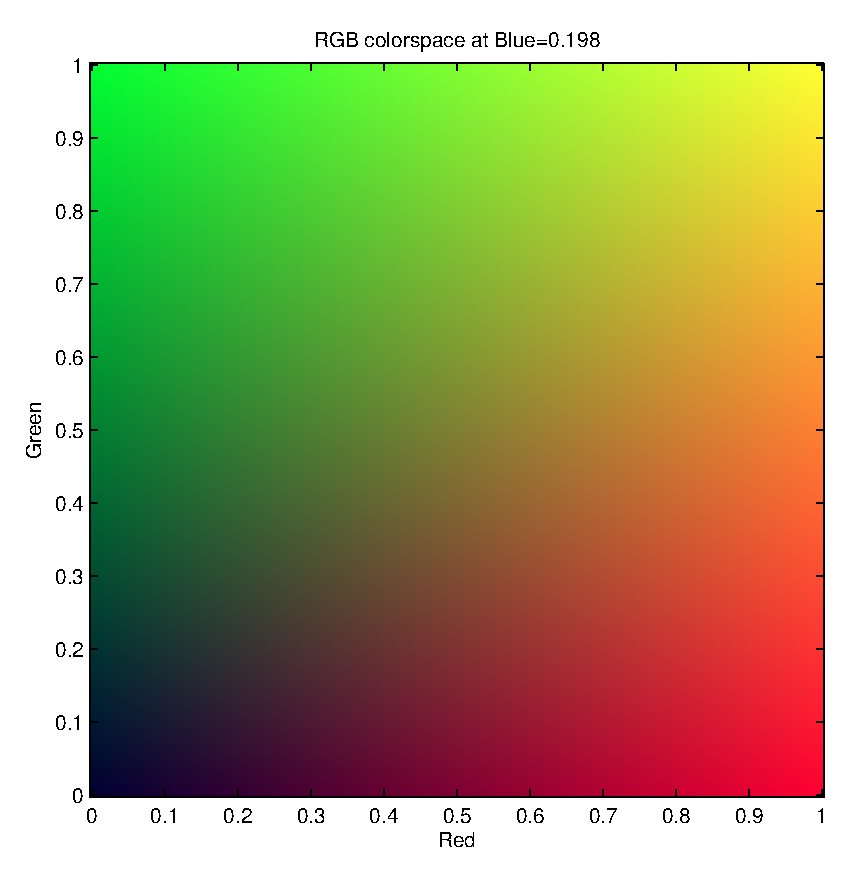
\includegraphics[width=0.45\textwidth]{bilder/colorspace}}
  \subfloat[RGB-färgrymden med ny
  basvektor]{\label{fig:rgbspace-base}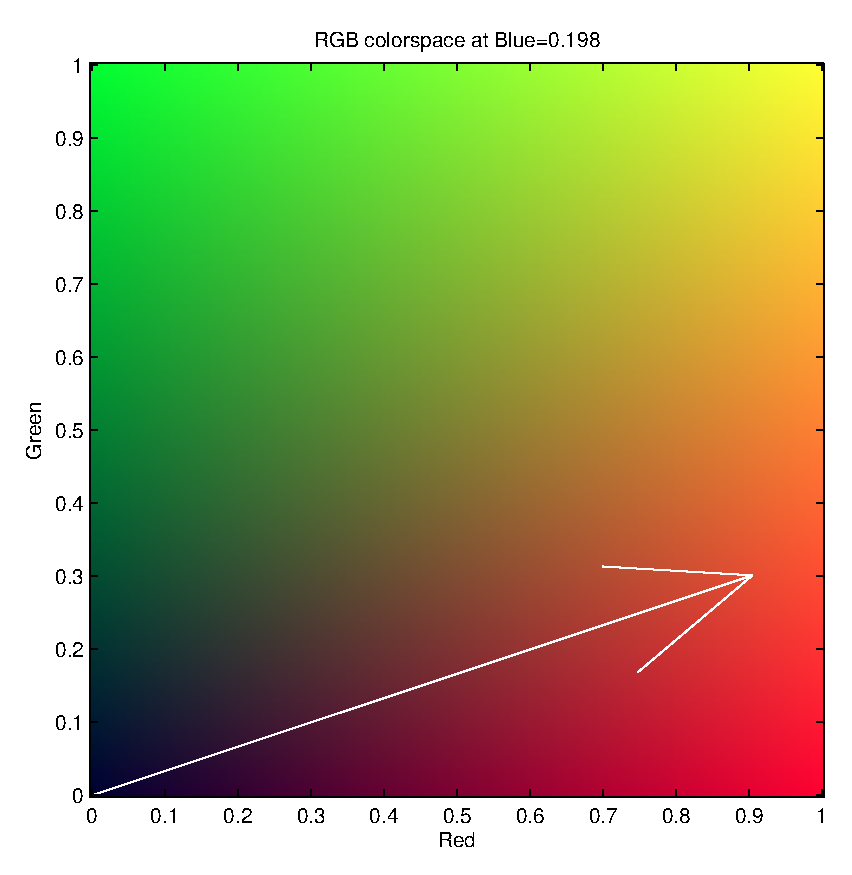
\includegraphics[width=0.45\textwidth]{bilder/colorspace_w_base}}\\
  \subfloat[RGB-färgrymden med nya
  basvektorer]{\label{fig:rgbspace-bchange}\includegraphics[width=0.7\textwidth]{bilder/colorspace_base_changed}}\\
  \caption{Processen för att ta fram en ny bas i färgrymden består av tre steg.}
  \label{fig:rgbspace}
\end{figure}

\end{document} 
